\section{The ChromoSSE Model} \label{sec:chromosse_intro}


A major challenge for all phylogenetic models of cladogenetic character change
is accounting
for unobserved speciation events due to lineages going extinct
and not leaving any extant descendants \citep{bokma2002detection},
or due to incomplete sampling of lineages in the present.
Teasing apart
the phylogenetic signal for cladogenetic and anagenetic processes given
unobserved speciation events is a major difficulty,
and using a naive approach that does not account for unobserved speciation
(like the ones discussed earlier in Section \ref{subsect:clado_simple}) 
can bias the relative rates of cladogenetic and anagenetic change.
The Cladogenetic State change Speciation and Extinction
(ClaSSE) model \citep{goldberg2012tempo}, on the other hand,
reduces this bias by explicitly incorporating unobserved speciation events.
This is achieved by jointly modeling both character evolution
and the phylogenetic birth-death process.
Not only does the ClaSSE framework enable the modeling of
unobserved speciation, but it also provides an easily extensible
framework for testing state-dependent speciation and extinction rates.


\begin{figure}[h!]
\fbox{
\begin{minipage}{\textwidth}\centering
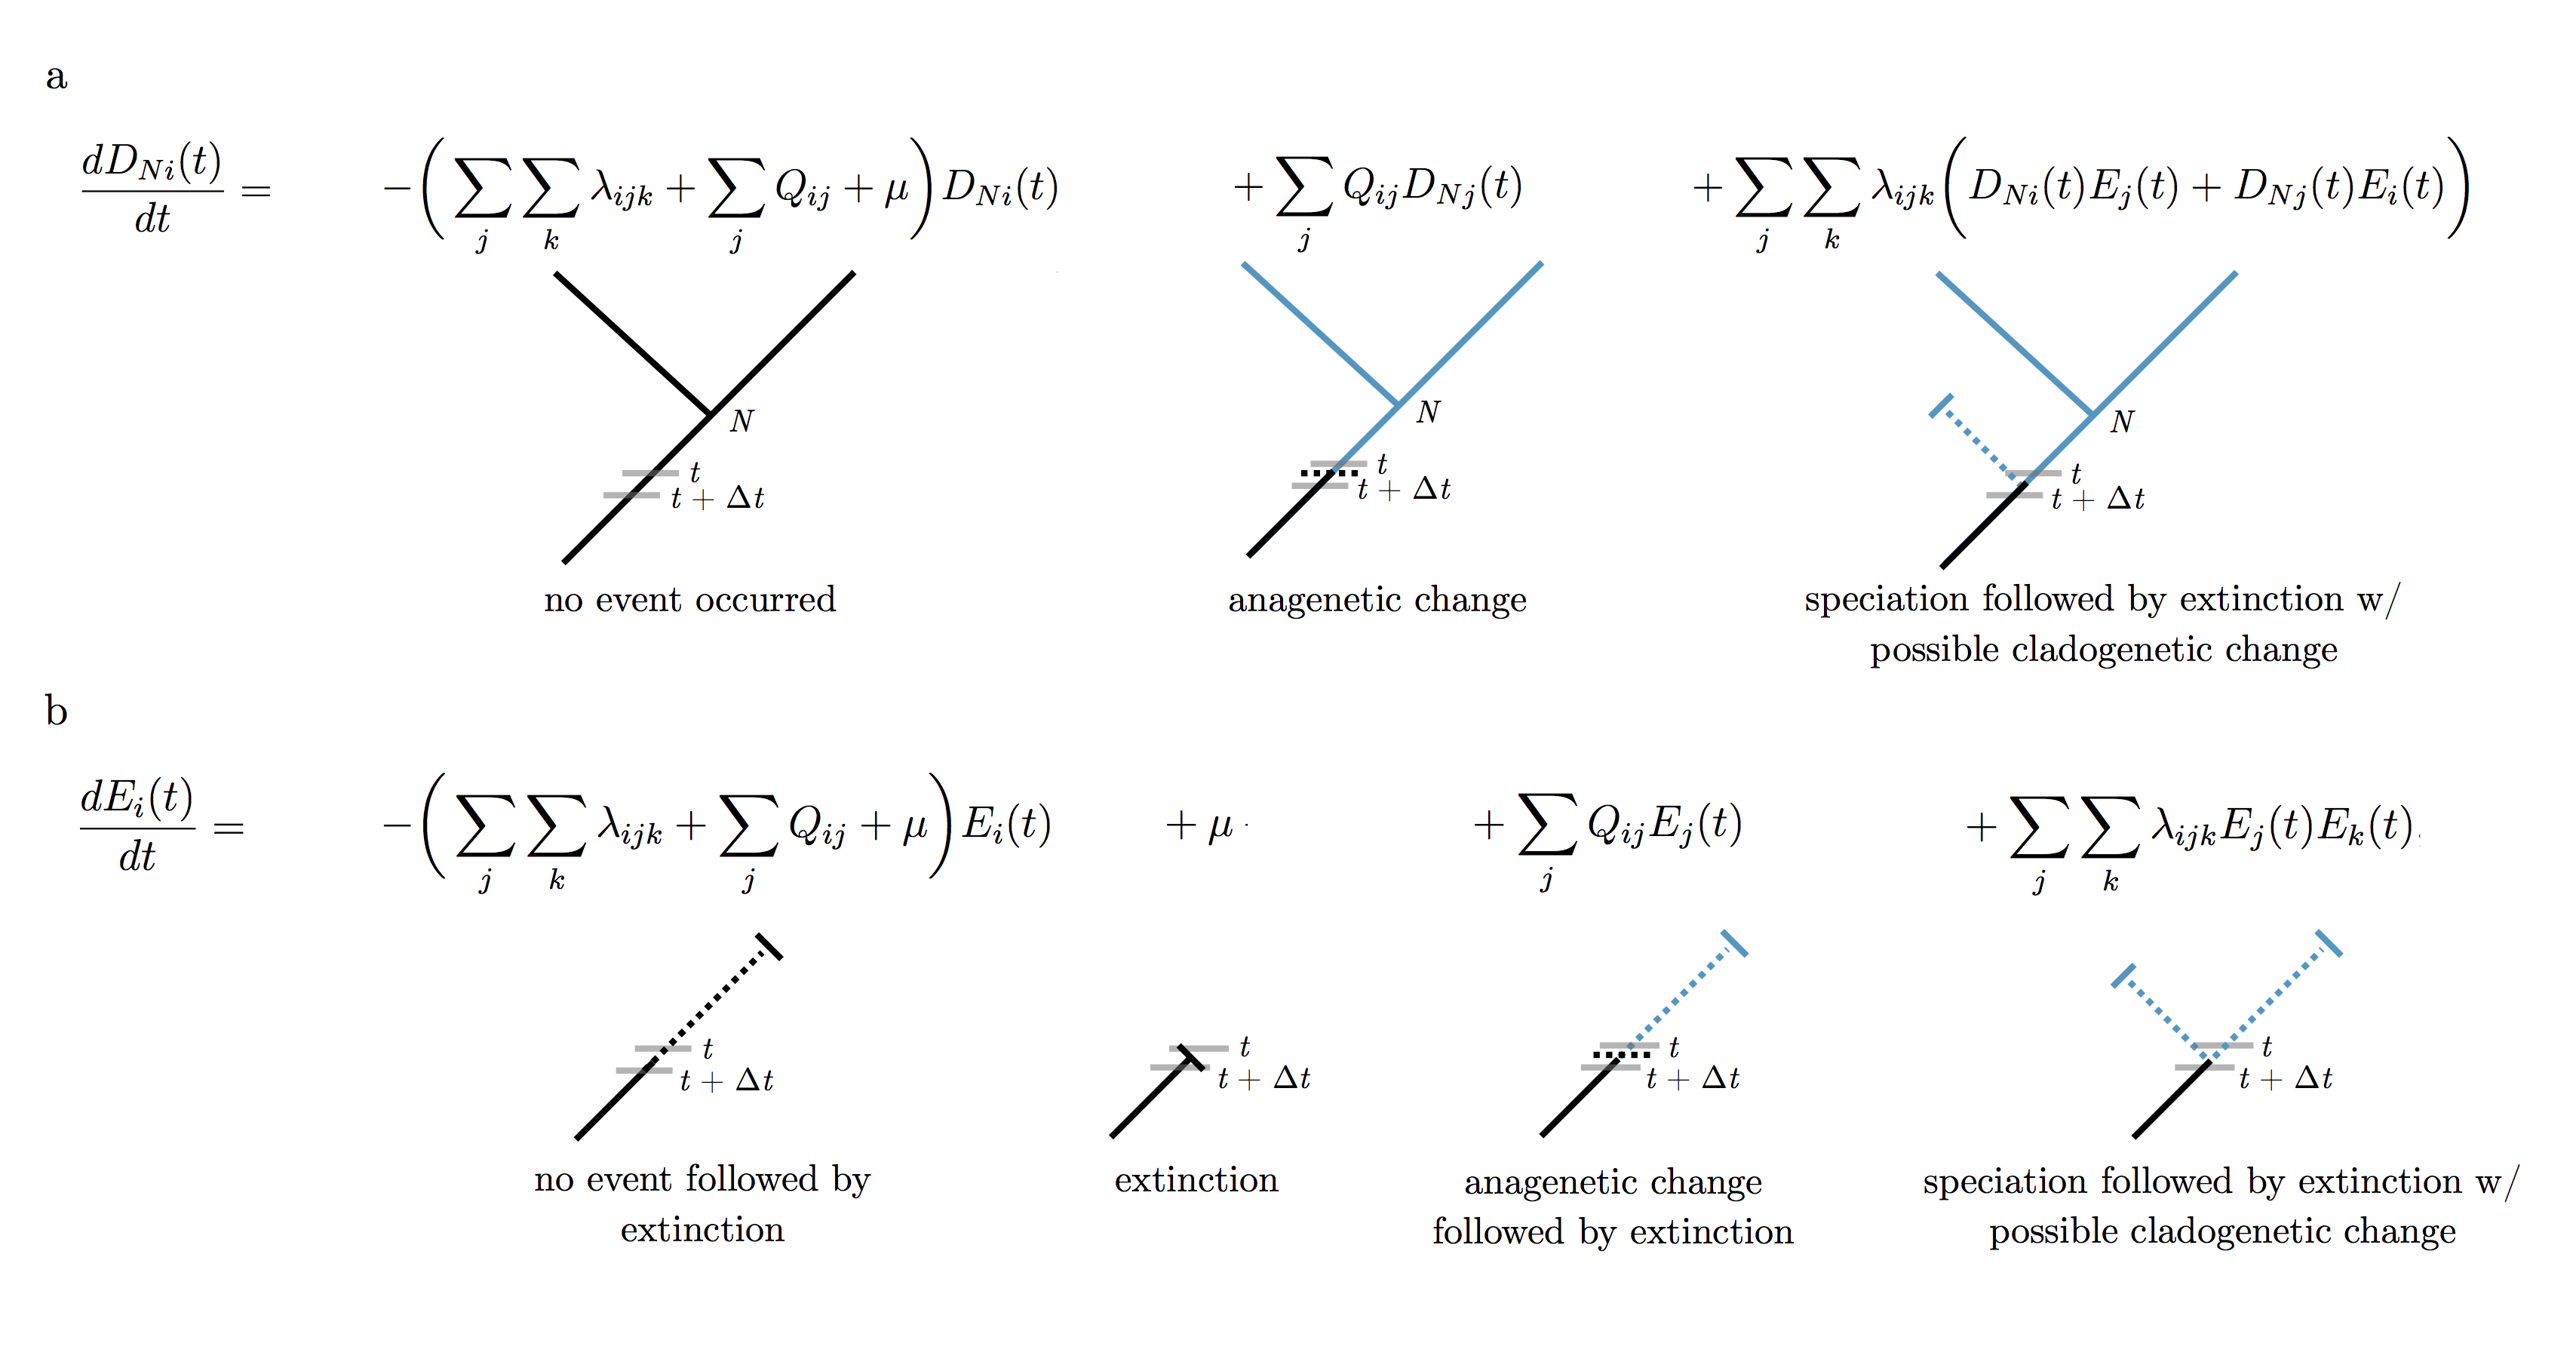
\includegraphics[trim={1cm 0cm 0.5cm 0cm},width=0.92\textwidth,angle=0]{\ResourcePath figures/ode_trimmed}
    \caption{
    An illustration of chromosome evolution events that could occur
    during each small time interval $\Delta t$ along the branches
    of a phylogeny as modeled in ChromoSSE \citep{freyman2016cladogenetic}.
    The set of differential equations
    (subfigures a and b, respectively)
    sum over each possible chromosome evolution event
    and are numerically integrated backwards through time
    over the phylogeny to calculate the likelihood.
    The transition rate matrix for anagenetic changes $Q$ 
    is explained in Section \ref{sec:chromo_basic_intro}.
    a) $D_{Ni}(t)$ is the probability that the lineage at time $t$
    evolves into the observed clade $N$.
    To calculate the change in this probability over $\Delta t$
    we sum over three possibilities: no event occurred,
    an anagenetic change in chromosome number occurred,
    or a speciation event with a possible cladogenetic chromosome change
    occurred followed by an extinction event on one of the
    two daughter lineages.
    b) $E_i(t)$ is the probability that the lineage
    goes extinct or is not sampled at the present.
    To calculate the change in this probability over $\Delta t$
    we sum over four possibilities:
    no event occurred followed eventually by extinction,
    extinction occurred,
    an anagenetic change occurred followed by extinction,
    or a speciation event with a possible cladogenetic change
    occurred followed by extinction of
    both daughter lineages.
    }
\end{minipage}}
\label{fig:chromosse_ode}
\end{figure}

The ChromoSSE model \citep{freyman2016cladogenetic} is a special case of the ClaSSE model that models chromosome changes.
Compared to the previously discussed CTMC models of chromosome evolution, SSE models require additional complexity since they must also
model the speciation and extinction process.
Simple extensions to the ChromoSSE model will enable explicit 
tests of different extinction rates for polyploid and diploid lineages,
and testing different rates of chromosome speciation associated with phenotypes or habitat.

\subsection{The ChromoSSE Likelihood Calculation}

All the previous models of chromosome number evolution discussed in the tutorial used
the standard pruning algorithm \citep{felsenstein81} to calculate
the likelihood of chromosome evolution over the phylogeny.
For the ChromoSSE model we must use a different approach;
here the likelihood is calculated using a set of ordinary differential
equations similar to the
Binary State Speciation and Extinction (BiSSE) model \citep{maddison2007estimating}.
The BiSSE model was extended to incorporate cladogenetic changes
by \citet{goldberg2012tempo}.
Following \citet{goldberg2012tempo}, we define
$D_{Ni}(t)$ as the probability that a lineage with
chromosome number $i$ at time $t$ evolves into the observed clade $N$.
We let $E_i(t)$ be the probability that a lineage
with chromosome number $i$ at time $t$ goes extinct before the present, or is not sampled at the present.
These two differential equations are shown and explained in Figure \ref{fig:chromosse_ode}.
However, unlike the full ClaSSE model the
extinction rate $\mu$ does not depend on the
chromosome number $i$ of the lineage.
This can easily be modified in \RevBayes to allow for different speciation and/or extinction rates
depending on ploidy or other character states.


\subsection{Next Steps}


In the next section we'll set up and run a \RevBayes analysis using the ChromoSSE model
of cladogenetic and anagenetic chromosome evolution.


\newpage
